\input{configuration}

\title{Lecture  34 --- Distributed Databases}

\author{Jeff Zarnett \\ \small \texttt{jzarnett@uwaterloo.ca}}
\institute{Department of Electrical and Computer Engineering \\
  University of Waterloo}
\date{\today}


\begin{document}

\begin{frame}
  \titlepage

 \end{frame}



\begin{frame}
\frametitle{Distributed Databases}

A distributed database is basically a scaled up shared nothing system. 

The database is stored on multiple computers and almost always at multiple physical locations.

 The systems that make up the distributed database need not be the same. 
 
  \end{frame}



\begin{frame}
\frametitle{Distributed Databases}

This is probably out of necessity: you can't order a computer with 4000 CPUs and 64~000 GB of RAM and 2000 hard drives, right? 

\begin{center}
	
\includegraphics[width=0.3\textwidth]{images/nomoon.jpg}
\end{center}
 
But you can order a thousand computers that each have 4 CPUS, that have 64~GB of RAM and 2 hard drives.

\end{frame}


\begin{frame}
\frametitle{Transparency}

When designing a distributed system one of the main concerns is \alert{transparency}. 

What we want is for it to be imperceptible to the users that the database is distributed.

\begin{center}
	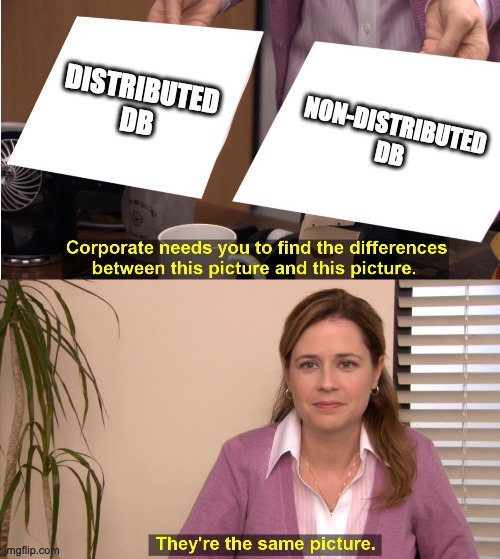
\includegraphics[width=0.4\textwidth]{images/samepicture.jpg}
\end{center}

\end{frame}


\begin{frame}
\frametitle{Transparency}

Types of transparency: 
\begin{itemize}
	\item \textbf{Location Transparency}
	\item \textbf{Naming Transparency}
	\item \textbf{Replication Transparency}
	\item \textbf{Fragmentation Transparency}
\end{itemize}



\end{frame}

\begin{frame}
\frametitle{Fragmentation}

Fragmentation is splitting up data. 

A relation $r$ can be divided up into arbitrarily many fragments $r_{1}, r_{2}, ..., r_{n}$.

Combining all the fragments allows reconstruction of the original relation $r$. 


\end{frame}


\begin{frame}
\frametitle{Horizontal Fragmentation}

In \alert{horizontal fragmentation}, each part of the relation $r_{i}$ contains some number of complete tuples. 

Each tuple is assigned to one or more fragments.

It does not mean that the tuples are inaccessible at other locations; they are just going to take longer to retrieve.

\end{frame}

\begin{frame}
\frametitle{Horizontal Fragmentation}

In relational algebra, a fragment $r_{i}$ is created by a selection with a predicate. 

So a fragment is $r_{i} = \sigma_{P_{i}}(r)$; the entire relation can be reconstructed as a union of the sets. 

This works only if the sets are disjoint -- no tuples are duplicated. 

\end{frame}


\begin{frame}
\frametitle{Horizontal Fragmentation}

\alert{Derived horizontal fragmentation} applies the partitioning of a relation rules to some secondary tables that are related by a foreign key. 

You have a relation that is a shipment and there is a related relation of containers. 

Some number of containers are associated with the shipment.

If a shipment is at location 1, its associated containers should also be there.

\end{frame}

\begin{frame}
\frametitle{Vertical Fragmentation}

\alert{Vertical fragmentation} is splitting up by attributes rather than tuples. 

In relational algebra fragmentation is done using projection: $r_{i} = \Pi_{R_{i}}
(r)$ and they are recombined using the natural join. 

For recombination to work, of course, we need a key in each part of the relation. If there are no attributes in common we have no way of recombining. 

\end{frame}



\begin{frame}
\frametitle{Hybrid Fragmentation}

\alert{Hybrid Fragmentation} is the all-of-the-above sort of fragmentation, where both horizontal and vertical fragmentation are applied. 

Recombination of the relation is accomplished by performing the union and outer join operations in the appropriate order.


\end{frame}

\begin{frame}
\frametitle{Replication}

\begin{center}
	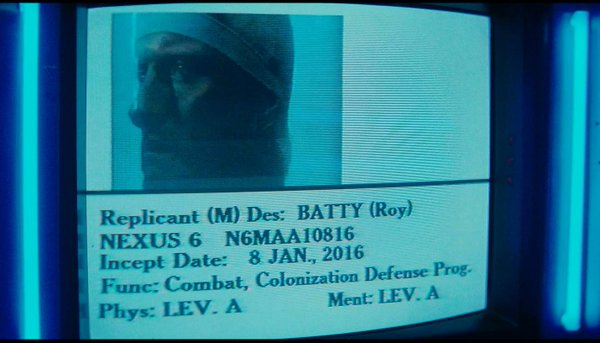
\includegraphics[width=0.75\textwidth]{images/roybatty.jpg}
\end{center}


\end{frame}

\begin{frame}
\frametitle{Replication}

Replication is making copies of the data available in different database servers. 

This may be to improve availability or reliability of data. 

At the one extreme, all data is replicated to all sites in the distributed system, meaning every location has all the data.

\end{frame}

\begin{frame}
\frametitle{Replication}

The simplest way to replicate is to not do it at all! 

There are no duplicate copies of the data and whatever fragment is at each location is the only copy. 

This means to get the full data, all systems must be online and available. 

\end{frame}


\begin{frame}
\frametitle{Replication}

If we do choose to replicate all of the data, then this is a fully-replicated distributed database.

The system can continue to function as long as any one location is operational.

It can improve performance of retrieval of data since we can always query the closest database. 

Unfortunately, it means much more work on an update since all locations have to be updated.

\end{frame}

\begin{frame}
\frametitle{Partial Replication}

In between is partial replication: some data is replicated over multiple sites and or all data is replicated in some way. 

A special case is when mobile workers go out into the field in areas where there is no internet connection.

\end{frame}


\begin{frame}
\frametitle{Replication}
Wherever data is replicated, we can choose one of the replicas to be the primary copy.

In databases under heavy load, replication is one of the keys to improving performance. 

\end{frame}


\begin{frame}
\frametitle{Replication}

A very common strategy is for reads to be done on replicas. 

One database is designated as the write master and all writes are done on the write master. 

The changes are then propagated to all replicas once the write is completed.


\end{frame}


\begin{frame}
\frametitle{Distributed Locking}

If we take the single lock manager approach, there is one single lock manager and one site is chosen as the leader. 

All requests are sent to that one site and that system tells the other system whether the request is granted, denied, or delayed. 

A read can be done at any one site that has the data, but a write requires all sites that have that data to participate.


\end{frame}


\begin{frame}
\frametitle{But Will It Scale?}

The single lock manager approach is simple in that there are only requests and responses and everything is managed centrally.

There is no need to invest effort to make sure that different lock managers agree. 

But there is the risk of failure at this one location causing the whole system to stop or misbehave.


\end{frame}

\begin{frame}
\frametitle{Distributed Lock Management}
If we choose instead to let all sites be involved in lock management, we have distributed lock management and the function is distributed. 

Immediately we can imagine this introduces the possibility that a disagreement arises about what data is locked and whether a lock can be granted.

But it does mean that we no longer are constrained by the single site. 

\end{frame}

\begin{frame}
\frametitle{Primary Copy}

A simple approach to distributed locking: the primary copy as controlling. 

If a site wishes to lock an item, it has to acquire the lock at the primary site. 

If a site goes down, the data for which it is the primary is inaccessible even though there is a replica of it (until some other site takes primary ownership).


\end{frame}

\begin{frame}
\frametitle{Majority Rules}

Majority protocol: if a data item $i$ is at $n$ different sites, then a lock message has to be sent to (at least) $\lceil n/2 \rceil$ locations to lock $i$. 

If a site finds according to its own local situation that the lock can be granted, it returns a yes answer immediately.

Otherwise the response is delayed until the lock can be acquired. 

A transaction on $i$ cannot proceed until a lock has been acquired on a majority of the locations.

\end{frame}


\begin{frame}
\frametitle{Majority Rules}

This routine requires a lot of messages. 

To lock an item requires $\lceil n/2 \rceil$ outgoing requests and also  $\lceil n/2 \rceil$ responses; to unlock an item then another $\lceil n/2 \rceil$ messages.

There is also the possibility of deadlock in this situation.

\end{frame}


\begin{frame}
\frametitle{Deadlock Sucks}

As you know, this occurs when there is a cycle in the resource requests. 

A transaction $T_{1}$ requests some item $i_{i}$ and then $i_{2}$ and a transaction $T_{2}$ requests $i_{2}$ then requests $i_{1}$. 

Under normal circumstances we can just require that data elements have to be requested in some predetermined order.

Unfortunately for us, in distributed systems this is not a guarantee.

\end{frame}


\begin{frame}
\frametitle{Biased Protocol}

Rather than treating every lock and unlock the same, we could make a distinction on shared vs. exclusive locks. 

In the biased protocol, to get a shared lock, we just need to request a shared lock on an item from any one site that has a replica of that item. 

To get an exclusive lock, a lock is requested from all sites that have the item.

\end{frame}


\begin{frame}
\frametitle{Biased Protocol}

If we expect that reads are more frequent than writes (this is very likely) then this is a performance increase. 

Reading any copy of the data can be done with just two messages, although a write requires $2n$ messages for each site where the data is stored. 

The request ordering problem is still at issue and the risk of deadlock still exists.

\end{frame}



\begin{frame}
\frametitle{Quorum Consensus Protocol}

In the \alert{quorum consensus protocol}, every site is assigned a weight (non-negative) and then to perform an operation enough sites need to agree. 

To execute a read, enough sites must agree such that their weights reach some threshold $r$. 

To execute a write enough sites must agree such that their weights reach a threshold $w$. 

The values for $r$ and $w$ can be the same or they can be set independently.

Why would we choose sites to have different weights? 

\end{frame}

\begin{frame}
\frametitle{Timestamp Protocol}

In the timestamp protocol, every transaction is assigned a unique timestamp. 

Each system uses its own local timestamp. 

Systems never agree on what time it is, so to make timestamps are unique, they are concatenated with the site identifier.

\begin{center}
\includegraphics[width=0.8\textwidth]{images/ddb-timestamp}
\end{center}

\end{frame}

\begin{frame}
\frametitle{Timestamp Protocol}
The placement of the site identifier in the concatenation is important! 

If we put it at the beginning then the timestamps at site $k$ would always appear to be after those of $k-1$ and before those of $k+1$, which would not be correct. 

A problem can still occur if the system timestamps are very far out of sync.

\end{frame}

\begin{frame}
\frametitle{Lazy Replication}
As a performance enhancement, databases may allow lazy replication.

Instead of having to do the write at all locations, we do write only at some location(s) and then the transactions get eventually transmitted to other sites.

Updates to an item are ordered serially because all updates to a single item take place at the same location. 

But other problems can occur such as an out-of-date value being used in a read as input to a write.

\end{frame}

\begin{frame}
\frametitle{Deadlock Detection}

A deadlock can occur but be difficult to detect using the wait-for graph algorithm, because nobody has the complete picture.

Each site may have its own local wait-for graph but that is not enough information to know if a deadlock has occurred.

\begin{center}
\includegraphics[width=0.75\textwidth]{images/waitfor-local}
\end{center}

\end{frame}

\begin{frame}
\frametitle{Put the Pieces Together}

If we combine the information we have the graph below, which does have a cycle:

\begin{center}
\includegraphics[width=0.5\textwidth]{images/waitfor-global}
\end{center}


\end{frame}

\begin{frame}
\frametitle{Global Wait-For Graph}

Our approach for solving this is the centralized approach.

One location is designated as deadlock coordinator and it is responsible for getting information from all other sites and aggregating it. 

The deadlock coordinator can then check this state and determine if there is a deadlock.

If so, use one of our resolution techniques to solve it.

\end{frame}

\begin{frame}
\frametitle{Running in and out of Time...}

The actual state of the system is not necessarily the same as the one seen by the deadlock coordinator. 

There is a potential communication delay between the various sites so the information reaching the coordinator can be out of date.

We might accidentally signal a rollback on a transaction that is not deadlocked.


\end{frame}

\begin{frame}
\frametitle{Checking for Deadlock}

Constantly checking the wait-for graph may be wasteful.

We might not even constantly send the wait-for graph information to the coordinator unless the coordinator asks for it.

What about if a transaction has been waiting a long time?

Other signs of a possible deadlock?

\end{frame}

\begin{frame}
\frametitle{Transaction Management}

In addition to the usual transaction management, there is the global transaction manager that is the boss of the other transaction managers. 

This may be a position where one database server holds the role permanently.

Or it might be that the database that handles the actual execution, or the one that started it.

\end{frame}

\begin{frame}
\frametitle{Why can't we all just get along?}

Our biggest concern is making sure that everyone agrees. 

At a fundamental level that means everyone needs to know about the transactions, and needs to agree about whether the transactions are committed or aborted. 

The first strategy we will examine is the two-phase commit protocol.

\end{frame}

\begin{frame}
\frametitle{Two Phase: Phase One}

A transaction is sent out to all the participating databases and they will do it.

In phase one, all databases signal the coordinator they are finished with actual execution.

When the coordinator has received that from all participating databases, it sends out a message telling all of them to prepare for commit.


\end{frame}

\begin{frame}
\frametitle{Two Phase: Prepare for Commit}

Then all the databases force write all log records and anything else the recovery process demands to disk. 

If all goes well they send back a signal saying OK; if something goes wrong they send back a signal that says ``Not OK''. 

If a timeout is reached without any response then a ``Not OK'' is assumed.

\end{frame}

\begin{frame}
\frametitle{Two Phase: Phase Two}

In phase two, if everyone said OK, and the coordinator also says OK, it sends a commit message to all the databases. 

Every database then proceeds with the commit. 

If something else happened, then the abort message is sent and all systems roll back the transaction. 

\end{frame}


\begin{frame}
\frametitle{Two Phase: All Done}

At the end of this, all systems have either committed or aborted the transaction and a consistent state is ensured whether the transaction succeeds or not. 

If a failure occurs during step one it usually results in rolling back, but if a failure occurs during phase 2 it usually results in commit.

\end{frame}

\begin{frame}
\frametitle{Two Phase Problems}

This protocol is good but it has some drawbacks. 

It is a blocking protocol; if the coordinator system fails, all the participating databases end up waiting until the coordinator system is back online. 

In the meantime they are locking data elements.

Alternatively, if a coordinator and participant that have committed crash together, then we might get an indeterminate result.

\end{frame}

\begin{frame}
\frametitle{MOAR PHASES!!!}

The proposed solution is the \alert{three phase locking protocol}. 

The third phase is added in between phase 1 and what previously was phase 2. 

The new second phase is that the coordinator shares with all participants the results of phase 2. 

Then phase 3 works just as the commit phase in the two-phase protocol.

\end{frame}

\begin{frame}
\frametitle{Three Phase}
If the coordinator crashes now, then some other participant can step up and take the coordinator role and see the transaction through. 

Thus, we can be sure the transaction will finish no matter what system crashes. 

This limits the wait time: based on the phase 1 information we know how the other systems will behave and we can just go ahead and commit. 

If no such message has been received, abort and proceed with other operations.

\end{frame}


\end{document}

